\section{Background}

\begin{frame}[c]{Natural Language Processing}
    \large
    \centering
    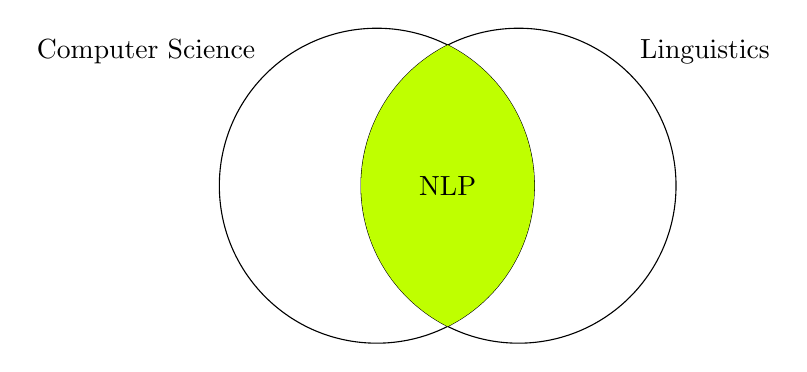
\begin{tikzpicture}

% Set A
\node [draw,
	circle,
	minimum size =4cm,
	label={135:Computer Science}] (A) at (0,0){};

% Set B
\node [draw,
	circle,
	minimum size =4cm,
	label={45:Linguistics}] (B) at (1.8,0){};

\scope % A \cap B
\clip (0,0) circle (2);
\fill[lime] (1.8,0) circle (2);
\endscope


% Set intersection label
\node at (0.9,0) {NLP};

    \end{tikzpicture} \\
    Goal: Make computers ``understand'' documents.
\end{frame}


\begin{frame}[c]{Information Extraction for Automated Experimentation}
    Information Extraction is the \gls{NLP} task of extracting structured (machine-readable) information from unstructured text.
    \begin{figure}
    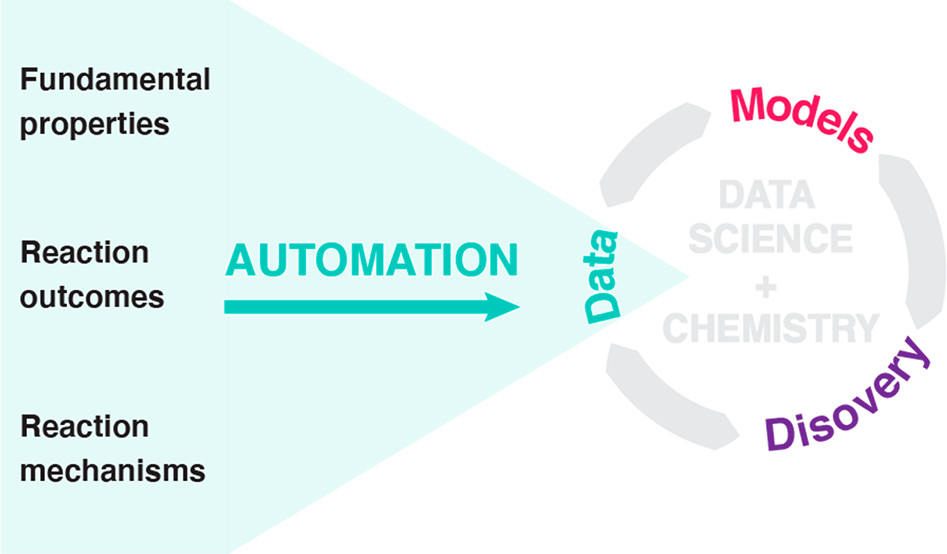
\includegraphics[height=0.55\textheight]{automated_experimentation}
    \caption{
    Image Source: \cite{shi_automated_2021}
    }
    \end{figure}
\end{frame}

\begin{frame}[c]{Namend Entity Recognition}
    \gls{NER} is the \gls{NLP} task of extracting structured (machine-readable) information from unstructured text.
    \begin{figure}
    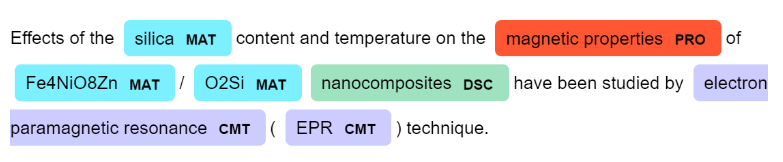
\includegraphics[width=\textwidth]{NER}
    \caption{
        \textbf{MAT} stands for Materials,
        \textbf{PRO} stands for Material Property,
        \textbf{DSC} is Descriptor and
        \textbf{CMT} is Characterization method.
        The goal of \gls{NER} is to automatically detect entities that fall into these pre-defined semantic types. \\
        Example and partial description taken from \cite{zhao_finetuning_2021} (supposedly taken from \cite{weston_named_2019}), visualized using the \texttt{spaCy} python library \cite{montaniispacy_natural_2017}.
    }
    \end{figure}
\end{frame}



\begin{frame}[c]{Rule-Based Entity Recognition}
    \large
    Easy: Regular Expressions! \pause
    ChemTagger \cite{hawizy_chemicaltagger_2011}, and others \cite{beard_comparative_2019, huang_database_2020} demonstrated that it works! \\
    \pause
    Except ...
    \begin{itemize}[<+(1)->]
        \item ``The mixture was filtered and the filterate was kept at \textit{room temperature} to obtained needle like colorless crystals of 1 after a month.'' \cite{vishnoi_flexible_2014}
        \item ``... distilled water, and dried at \textit{ambient temperature} to give 39 mg of ...'' \cite{lin_new_2005}
        \item ``... was added into 1 mL \textit{boiling methanol solution} of btpe ...'' \cite{wang_two_2012}
        \item ...
    \end{itemize}
\end{frame}


\begin{frame}[c]{Language Models for Information Extraction}
    \begin{figure}
        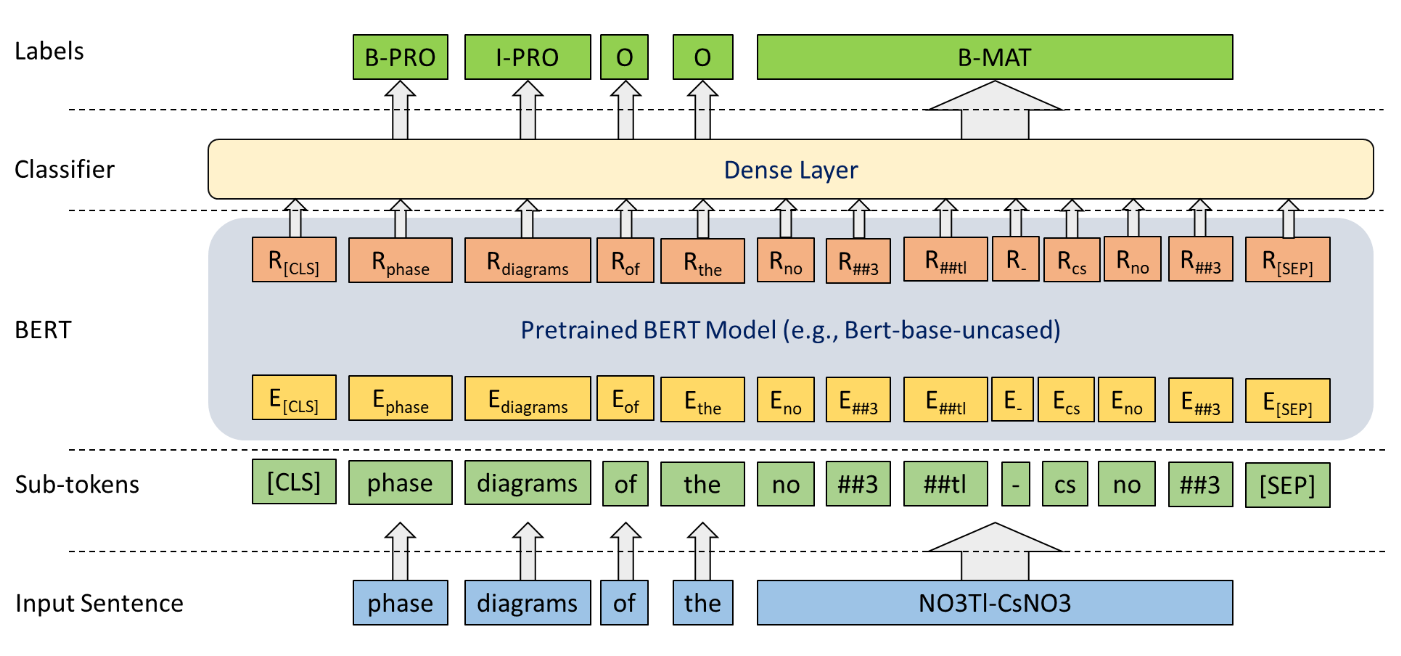
\includegraphics[height=0.6\textheight]{BERT_NER}
        \caption{
            \gls{NER} modeled as a sequence-to-sequence labeling problem can achieve high accuracy using \gls{BERT}-based
            \glspl{LM}. Image Source: \cite{zhao_finetuning_2021}
        }
    \end{figure}

\end{frame}

\begin{frame}[c]{Large Language Models for Structured Information Extraction}
    \begin{figure}
        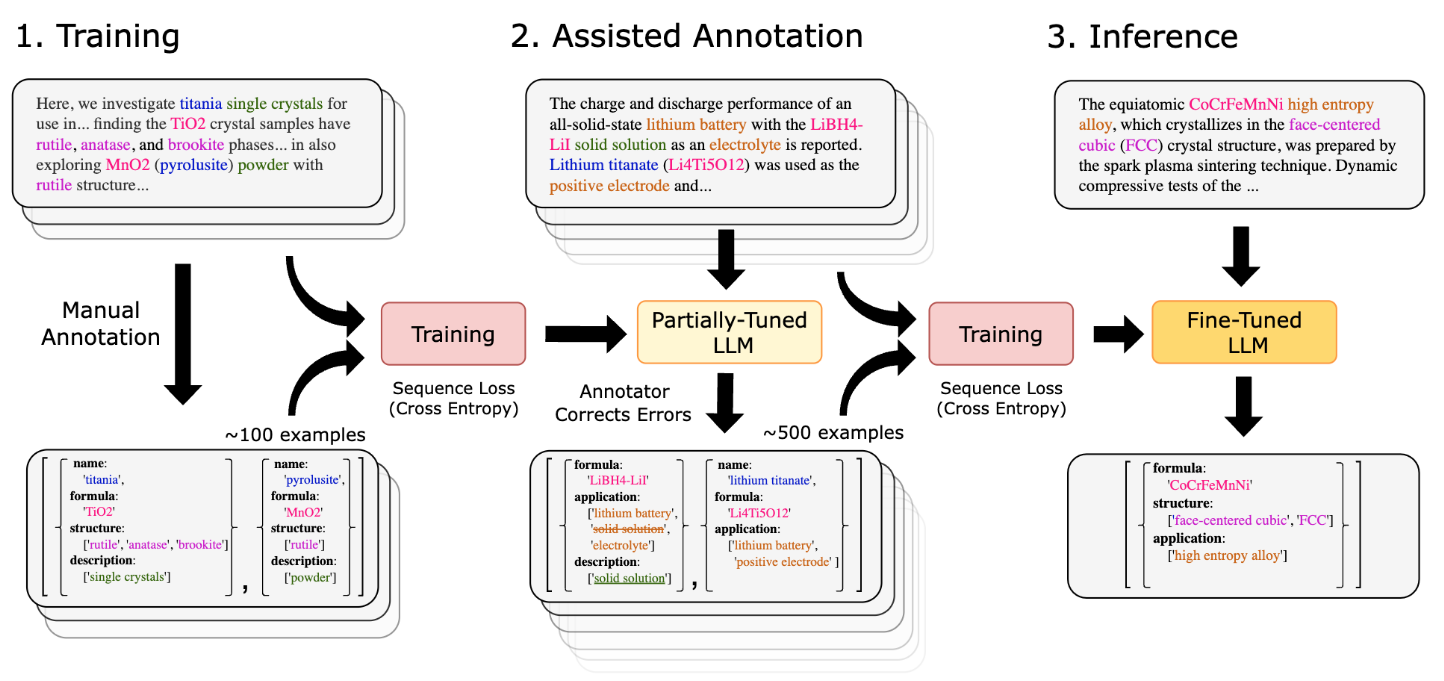
\includegraphics[height=0.6\textheight]{finetuned_llm_er}
        \caption{
            Other work focused on Entity Relation extraction, with mixed results for \gls{NER}. \\
            Image Source: \cite{dunn_structured_2022}
        }
    \end{figure}
\end{frame}

